\documentclass{scaffold/sigchi}
\usepackage{pifont} % Check marks
\newcommand{\cmark}{\ding{51}} % So we can use \cmark instead of \ding{51}
\newcommand{\xmark}{\ding{55}}
\usepackage[none]{hyphenat}
\bibliographystyle{unsrt}


% Title
\def\plaintitle{Investigating How Different Modalities of Positive Reinforcement Influence the Formation of New Habits}

% Authors as plain text
\def\plainauthor{First Author, Second Author, Third Author,
  Fourth Author, Fifth Author, Sixth Author}
\def\emptyauthor{}
\def\plainkeywords{habit formation; habit automaticity; behaviour change; chatbot; rewards; modalities; visual; auditory; visual-auditory.}
\def\plaingeneralterms{Documentation, Standardization}
  \usepackage{pgfplots}
  \pgfplotsset{compat=1.12}

% Use this section to set the ACM copyright statement (e.g. for
% preprints).  Consult the conference website for the camera-ready
% copyright statement.

% Copyright
\CopyrightYear{2017}
%\setcopyright{acmcopyright}
\setcopyright{acmlicensed}
%\setcopyright{rightsretained}
%\setcopyright{usgov}
%\setcopyright{usgovmixed}
%\setcopyright{cagov}
%\setcopyright{cagovmixed}
% DOI
\doi{http://dx.doi.org/10.475/123_4}
% ISBN
\isbn{123-4567-24-567/08/06}
%Conference
\conferenceinfo{CHI'18,}{April 21--26, 2018, Montreal, Canada}
%Price
% \acmPrice{\$15.00}

% Use this command to override the default ACM copyright statement
% (e.g. for preprints).  Consult the conference website for the
% camera-ready copyright statement.

%% HOW TO OVERRIDE THE DEFAULT COPYRIGHT STRIP --
%% Please note you need to make sure the copy for your specific
%% license is used here!
% \toappear{
% Permission to make digital or hard copies of all or part of this work
% for personal or classroom use is granted without fee provided that
% copies are not made or distributed for profit or commercial advantage
% and that copies bear this notice and the full citation on the first
% page. Copyrights for components of this work owned by others than ACM
% must be honored. Abstracting with credit is permitted. To copy
% otherwise, or republish, to post on servers or to redistribute to
% lists, requires prior specific permission and/or a fee. Request
% permissions from \href{mailto:Permissions@acm.org}{Permissions@acm.org}. \\
% \emph{CHI '16},  May 07--12, 2016, San Jose, CA, USA \\
% ACM xxx-x-xxxx-xxxx-x/xx/xx\ldots \$15.00 \\
% DOI: \url{http://dx.doi.org/xx.xxxx/xxxxxxx.xxxxxxx}
% }

% Arabic page numbers for submission.  Remove this line to eliminate
% page numbers for the camera ready copy
% \pagenumbering{arabic}

% Load basic packages
\usepackage{balance}       % to better equalize the last page
\usepackage{graphics}      % for EPS, load graphicx instead 
\usepackage[T1]{fontenc}   % for umlauts and other diaeresis
\usepackage{txfonts}
\usepackage{mathptmx}
\usepackage[pdflang={en-US},pdftex]{hyperref}
\usepackage{color}
\usepackage{booktabs}
\usepackage{textcomp}

% Some optional stuff you might like/need.
\usepackage{microtype}        % Improved Tracking and Kerning
% \usepackage[all]{hypcap}    % Fixes bug in hyperref caption linking
\usepackage{ccicons}          % Cite your images correctly!
% \usepackage[utf8]{inputenc} % for a UTF8 editor only

% If you want to use todo notes, marginpars etc. during creation of
% your draft document, you have to enable the "chi_draft" option for
% the document class. To do this, change the very first line to:
% "\documentclass[chi_draft]{sigchi}". You can then place todo notes
% by using the "\todo{...}"  command. Make sure to disable the draft
% option again before submitting your final document.
\usepackage{todonotes}






% llt: Define a global style for URLs, rather that the default one
\makeatletter
\def\url@leostyle{%
  \@ifundefined{selectfont}{
    \def\UrlFont{\sf}
  }{
    \def\UrlFont{\small\bf\ttfamily}
  }}
\makeatother
\urlstyle{leo}




% To make various LaTeX processors do the right thing with page size.
\def\pprw{8.5in}
\def\pprh{11in}
\special{papersize=\pprw,\pprh}
\setlength{\paperwidth}{\pprw}
\setlength{\paperheight}{\pprh}
\setlength{\pdfpagewidth}{\pprw}
\setlength{\pdfpageheight}{\pprh}

% Make sure hyperref comes last of your loaded packages, to give it a
% fighting chance of not being over-written, since its job is to
% redefine many LaTeX commands.
\definecolor{linkColor}{RGB}{6,125,233}
\hypersetup{%
  pdftitle={\plaintitle},
% Use \plainauthor for final version.
%  pdfauthor={\plainauthor},
  pdfauthor={\emptyauthor},
  pdfkeywords={\plainkeywords},
  pdfdisplaydoctitle=true, % For Accessibility
  bookmarksnumbered,
  pdfstartview={FitH},
  colorlinks,
  citecolor=black,
  filecolor=black,
  linkcolor=black,
  urlcolor=linkColor,
  breaklinks=true,
  hypertexnames=false
}

% create a shortcut to typeset table headings
% \newcommand\tabhead[1]{\small\textbf{#1}}

\title{\plaintitle}




% Authors on paper
\numberofauthors{3}
\author{%
  \alignauthor{Leave Authors Anonymous\\
    \affaddr{for Submission}\\
    \affaddr{City, Country}\\
    \email{e-mail address}}\\
  \alignauthor{Leave Authors Anonymous\\
    \affaddr{for Submission}\\
    \affaddr{City, Country}\\
    \email{e-mail address}}\\
  \alignauthor{Leave Authors Anonymous\\
    \affaddr{for Submission}\\
    \affaddr{City, Country}\\
    \email{e-mail address}}\\
}

\begin{document}

\maketitle

\begin{abstract}
Rewards motivate people to complete actions. Habit formation systems use rewards to motivate people to form habits. This paper looks at the effect of three types of positive reinforcement rewards on habit formation delivered by a chatbot, from three modes: visual, auditory and visual-auditory combined. The findings are evaluated against two hypotheses: i) rewards effect on habit performance and automaticity, ii) multiple modalities effect on habit performance and automaticity. 60 people participated in a 4-week study followed by voluntary semi-structured interviews. The findings showed that participants receiving the bot-delivered rewards had higher habit performance than the control group without rewards. A correlation was found between the habit formation method and habit automaticity. However, all participants interviewed (N = 7) found a drop in habit performance after one week without the prototype. Further research for using different rewards with behaviour change technology is needed to validate how each modality affected habit automaticity and habit performance.
\end{abstract}

\category{H.5.2}{Information interfaces and presentation (e.g. HCI)}{User Interfaces, auditory (non-speech) feedback, interaction styles, miscellaneous}

\keywords{\plainkeywords}


\section{Introduction}
Understanding how to design systems that support behaviour change is important to human computer interaction (HCI) to ensure that designers build these systems to have the maximum impact~\cite{how_to_evaluate_tech_for_behaviour_change}. Habits play an important role in behaviour change by making the changed behaviour permanent~\cite{article_promoting_habit_formation}. However, the full habit formation process within the HCI domain needs further research due to the difficulties in evaluating the long-term effects of technology on habit formation~\cite{article_evaluate_tech_health_behaviour_change}. Therefore, the need for HCI researchers to design technology that encourages people to change their behaviour and form new habits is still a main focus.

Habits are automatic actions that require little concious effort~\cite{article_the_habitual_consumer}. To develop new habits people must keep to a strict routine and perform the action repeatedly to strengthen the automaticity of the action~\cite{article_promoting_habit_formation}. When strong habits are developed the likelihood of behaviours persisting is higher~\cite{putting_habit_into_practice} and habits are more effectively developed when specific and measurable goals are set~\cite{habits_better_when_have_specific_and_measurable_goals}. Psychology defines habits as learned automatic cue-response actions. The action will perform automatically in response to a trigger that has been actioned repeatedly in the past~\cite{article_the_habitual_consumer}. The more automatic the response the higher habit automaticity. For example, a simple action such as turning on the light when you enter a room, happens automatically, even if the light is already on. However, forming a new habit is difficult and people are more likely to give up due to their lack of routine~\cite{article_promoting_habit_formation, article_the_habitual_consumer}.

Technology can help people stick to a routine by sending repeated messages~\cite{chi_crowd_designed_motivation} and encouraging people~\cite{positive_reinforcement_pro}. However, these techniques do not always work and may build repetitive actions rather than habit automaticity~\cite{coaching_not_that_good}. Therefore, technology should be designed to avoid building repetitive actions and instead build habit automaticity. Repetitive actions lead people to become dependent on technology and when the system is eventually removed, habit performance decreases~\cite{article_dont_kick_habit, article_realtime_feedback_improving_medication_taking}. Habit automaticity is a measure of habit strength~\cite{article_4q_SRBAI} and is the key that removes this dependency~\cite{article_beyond_self_tracking_designing_apps}. Automaticity can be increased by building motivation to complete the action~\cite{article_a_self_efficacy, article_meta_analytic_review_intrinsic_motivation}.
Motivation can be encouraged by giving people positive reinforcement rewards after they complete an action. However, how the reward is delivered and the type of reward used is also crucial to success.

The method of delivery should suit each individual user and a choice of delivery should be available. For example, a survey on feedback systems~\cite{article_user_centred_multimodal_reminders} advised that delivery of interaction should span different modalities to increase retention and better suit the needs of users. Although interaction across modalities is important, this research does not have configurable feedback, but aims to compare how each type of feedback can affect motivation. Monetary (extrinsic) rewards can hinder motivation~\cite{article_meta_analytic_review_intrinsic_motivation}, whereas, satisfaction-based (intrinsic) rewards can be beneficial to motivation and should be preferred. 
This study uses a chatbot to deliver intrinsic positive reinforcement rewards from different modalities to see how participants habit automaticity and performance are affected.

This paper is comprised of three sections. First, an analysis of a 4-week situated study measuring the impact of visual, auditory and visual-auditory rewards on participants habit automaticity and the number of habits completed. Second, a demonstration of how the bot-delivered rewards encourage people to stick to a routine and perform their habit. Finally, the effect of tracking habits on habit automaticity is looked at and the dependency issues arising with technology and habit formation are discussed.

\section{Background}
To understand how to build a tool to support habit formation, we must discuss how people fundamentally form habits and the impact of each reward modality.

\subsection{Habit Formation}
The formation of new habits requires behaviour change. Three elements are needed to make this change permanent: contextual cues, repetition and positive reinforcement~\cite{article_experiences_of_habit_formation}. However, people still fail at forming new positive habits and give up, often due to their lack of routine~\cite{article_promoting_habit_formation, article_the_habitual_consumer}.

\subsubsection{Cues and Repetition}
The process of creating a new habit takes constant repetitive use~\cite{article_how_habits_formed_modelling_habit_formation}. The easier the action, the shorter the time before the action turns into a habit, from drinking water (18 days), to going to the gym (254 days). However, existing routines and cues are needed before the action develops into a habit~\cite{habits_event_cues_1, habits_event_cues_2}. An existing routine acts as a trigger to motivate the desired action. Context from that routine serves as the cue for the trigger. For example, if you wanted to adopt a habit to weigh yourself every day, you could attach it onto an existing habit like brushing your teeth. The contextual cue of brushing your teeth will trigger you to weigh yourself. When designing behaviour change interventions, using different types of cues can be beneficial. Multi-cue routines have shown to be more effective than a single cue~\cite{article_understanding_use_contextual_cues_design_impl}. Attaching habits onto existing event-based cues are easier to remember~\cite{article_implementation_intentions_multicue} when compared with time-based habits, mainly due to change in time with change in environment, e.g. the weekend~\cite{coaching_not_that_good}. Event-based cues help connect the contextual information with the action and builds habit automaticity~\cite{article_implementation_intentions}.
 
\subsubsection{Rewards}
Rewards give motivation, fuelling the belief in success and self-efficacy, which plays a large part in forming habits. Some researchers~\cite{article_a_self_efficacy} suggest it is the main part of behaviour change. Variable types of rewards have been shown to increase dopamine in a laboratory study on rats~\cite{variable_rewards_increases_dopamine}. This technique has proved to be an effective method of increasing repetition as shown in slot machines that vary their reward payout. But although variable rewards increase habit repetition, they hinder habit automaticity~\cite{variable_rewards_increases_dopamine}, which is key to creating permanent and long-lasting behaviour change. Rewards are a good form of external motivation because they don't change the ability to perform a behaviour, unless the reward itself is a tool that increases ability~\cite{article_taxonomy_motivational_affordances_meaningful}. Rewards provide a strong motivational source, but like all extrinsic motivators, these are less effective for changing behaviour in the long run, because externally motivated behaviour lasts as long as the external motivator exists~\cite{article_beyond_self_tracking_designing_apps}.


\subsection{Positive Reinforcement}
Positive reinforcement rewards the person by encouraging them to perform the action again until it forms into a habit. Research~\cite{positive_reinforcement_pro} has shown that positive reinforcement significantly increases intrinsic motivation and increases the persons perception of their own performance. This paper discusses intrinsic positive reinforcement as the method of reward, rather than other types of rewards e.g. negative reinforcement. Rewarding a person with intrinsic positive reinforcement strengthens the habit by giving the feeling of satisfaction~\cite{article_promoting_habit_formation}, particularly in relation to interesting tasks~\cite{article_meta_analytic_review_intrinsic_motivation}. This study explores different types of positive reinforcement rewards and how they effect behaviour change.

\subsection{Modalities}
The three chosen modes, visual, auditory, and visual-auditory combined, are chosen for testing. Feedback from each of these different modalities has been shown to improve task performance for small tasks~\cite{chi_oussama_tap_the_shapetones}. Combining modalities can be useful for issuing user feedback, enabling systems to be accessible to varying ages~\cite{article_user_centred_multimodal_reminders}. Individual modes can improve the effectiveness of reminders~\cite{multi_modal_reminders_less_disruptive, article_designing_multimodal_reminders_for_home}. However, the effectiveness of each type of modality as reward feedback and how combined modalities affect interaction has little research. Therefore, technology to support behaviour change should explore a range of modalities and feedback should not be annoying as positive reinforcement should be a satisfactory experience. Research into visual, auditory and visual-auditory feedback was identified to understand how they impact behaviour to see how habit formation is impacted.

\subsubsection{Visual}
Visual feedback can encourage task performance consistency as demonstrated in one study by Lee et al.~\cite{article_realtime_feedback_improving_medication_taking} where they constructed a device that gave constant visual feedback for patients taking medication. They found that visual feedback improved consistency of the habit and increased the rate of self-efficacy. But when the device was removed, their performance dropped (as measured after a 2-month period). This suggests that users did integrate the visual feedback display cue with their routines, but they also became dependant on the technology and the visual feedback did not build habit strength. Users should instead build these cues outside of the system, with another routine to build habit automaticity and allowing for permanent behaviour change after the system is removed.

\subsubsection{Auditory}
There is a need to use audio when designing for behaviour change technology, especially with a varied target market~\cite{article_designing_for_health_behaviour_change_hci}. For example, combining different sounds for different actions to suit different users~\cite{article_movipill_improving_medication_elders}. Using auditory as a method of delivery has shown to improve task success~\cite{auditory_notifications_increase_delivery_success}, but little work has shown how it impacts habit performance.

\subsubsection{Visual-Auditory}
Several studies show that combining audio with visual as feedback after the completion of a simple task, can be successful~\cite{benefits_of_audio_visual_1, benefits_of_audio_visual_2}. A meta-analysis of 43 multi-modal studies~\cite{comparing_modalities_effects_of_visual_auditory} revealed that it was the most effective to increase performance, when a single task is being performed and when compared with visual or auditory feedback alone. Additional research shows this combination of visual and auditory sensory channels has been shown to increase performance with complex tasks~\cite{chi_oussama_tap_the_shapetones}. However, care needs to be taken when adding an extra modality as this study showed that '\textit{visual feedback improved task performance, but sacrificed task quality}'~\cite{comparing_modalities_effects_of_visual_auditory}. In addition, while all modalities contribute to perceptual experience, one sense can override another if the sensory channel mediates less ambiguous information than the other~\cite{one_mode_override_another}. Therefore it will be useful to compare the success of the task with the other modes. Using a combination of modalities for interaction gives a means of communication to people with varying levels of sensory awareness. 

\subsection{Technology}
Research~\cite{survey_on_apps_2,survey_on_current_apps_of_steel} into how technology can support habit formation and behaviour change, shows a large number of habit forming systems are mobile apps. Studies into the effectiveness of these apps has been recently conducted~\cite{article_beyond_self_tracking_designing_apps, article_dont_kick_habit} revealing that although most of these apps are rated highly, they do not ground themselves in behaviour change theory. Further surveys of these apps~\cite{survey_on_current_apps_of_steel,survey_on_apps_2} suggest that habit performance is not sustained when the app is removed, due to the lack of habit automaticity built during the habit tracking process. Using apps consistently to manage behaviour can create a notable difference in the person when the system is removed~\cite{article_my_phone_is_part_of_my_soul}.
This is also the case with many behaviour change systems, when the system is removed any improved performance is lost~\cite{article_dont_kick_habit, article_realtime_feedback_improving_medication_taking}.


\begin{figure}
  \centering
  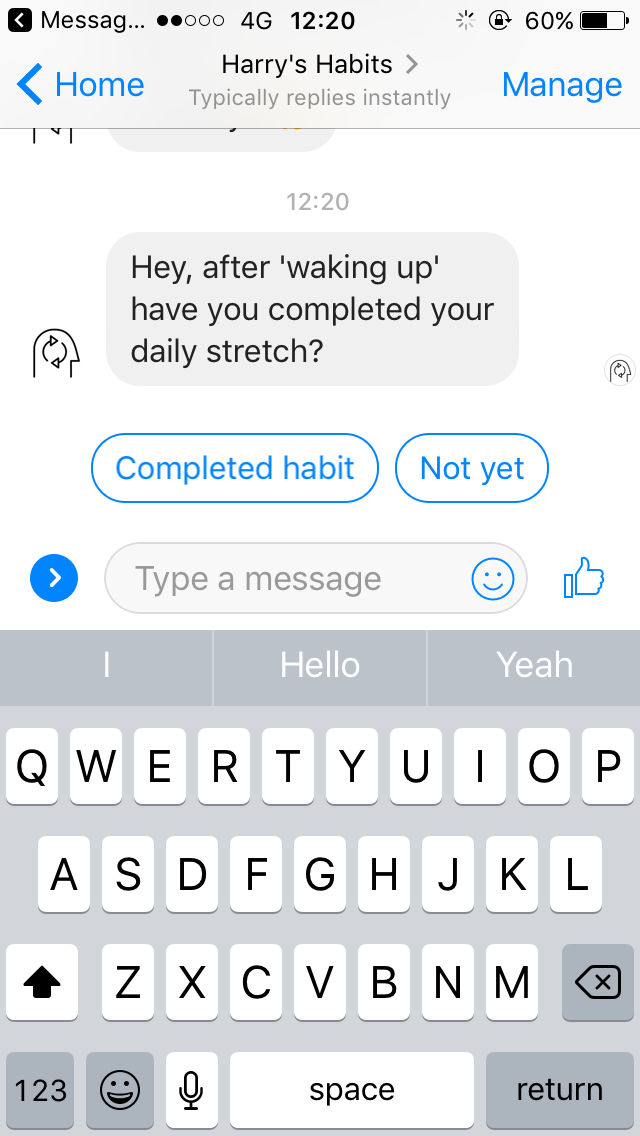
\includegraphics[width=0.47\columnwidth]{figures/reminder.png}
  \hspace{5px}
  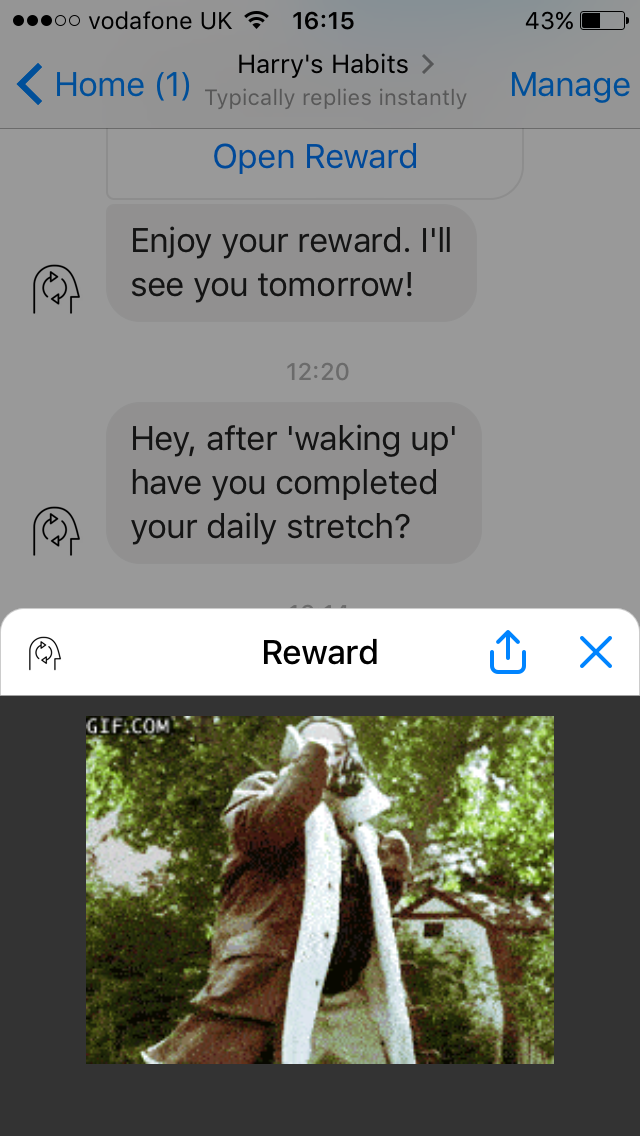
\includegraphics[width=0.47\columnwidth]{figures/reward-visual.png}
  \caption{Prototype delivering a visual reward after a user has marked their habit as completed.}~\label{fig:setup}
\end{figure}

\section{Study: Comparing Different Rewards}
To explore the influence of different modalities on habit formation, a situated study was conducted, followed by semi-structured interviews. For the purpose of the study a chatbot was developed to help users form healthy habits by providing different types of positive reinforcement. The study and the bot itself are described below.

\subsection{Hypotheses and Measurements}
The study tests two hypotheses, the effect of the rewards and the effect of multiple modes versus singular modes. They are measured by habit performance and habit automaticity.

\subsubsection{M1: Habit Performance}
The number of habits a participant marked as completed, incremented when a participant presses '\textit{completed habit}' on the bot.

\begin{itemize}
	\item \textit{M1H1: The rewards effect on habit performance}
	\item \textit{M1H2: Multiple modes versus singular on habit performance}
\end{itemize}

\subsubsection{M2: Habit Automaticity}
Calculated from two Self-Report Behavioural Automaticity Index (SRBAI)~\cite{article_4q_SRBAI} questionnaires and feedback from participant interviews.
\begin{itemize}
\item \textit{M2H1: The rewards effect on habit automaticity}
\item \textit{M2H2: Multiple modes versus singular on habit automaticity}
\end{itemize}

\subsection{Method}
The study aims to test the hypotheses comparing how well people form new habits based on the rewards and how the bot-delivered rewards effect participants habit formation.

\subsubsection{Chatbot}
Several systems were reviewed to test their feasibility as a prototype. A chatbot was chosen as it: can easily send notifications, is cross-platform, therefore highly available and is simple, with the user interface (UI) already constructed. The bot was custom built and designed to track participants habits and deliver the rewards. The rise of social media and increasing use of humorous memes was utilised to provide the motivating content of the rewards (Figure~\ref{fig:setup}). This works well with the prototype integration into an existing social media messaging platform \textit{Facebook Messenger} (\url{www.messenger.com}) participants were used to, therefore the social scaffolding around the interaction will help reinforce the response to notifications and logging of habit behaviour~\cite{the_power_of_logging_mobile_notifications} as participants are more likely to respond because participants perceive the bot as a real person because it is located next to other real people.


\subsubsection{Participants}
60 participants were recruited with public posts to social networks and were mostly University students and staff.

\subsubsection{Design}
Participants were instructed to connect with the bot via Facebook Messenger and pick a series of options to set-up their habit tracking. A brief description accompanied these options, to guide the participants on how to answer. The habits participants could choose were split into two categories, physical and relaxation. They were: stretching, press ups, the plank, reading, writing or meditation. Participants were aware of these habits before they consented to the study and if they did not want to form any of these habits they would not start the study. These simple actions were chosen to match the length of the study, as simple tasks become automatic quicker than complex actions~\cite{article_how_habits_formed_modelling_habit_formation}, for example a drinking water habit only takes, on average, 18 days of repetitive use.

The study used four conditions: visual rewards, auditory rewards, visual-auditory rewards and no rewards (control group). Participants were randomly assigned a condition by the bot after they completed the set-up, 15 were assigned to visual rewards, 15 assigned to auditory rewards, 15 assigned to visual-auditory rewards and 15 with no rewards (control group). The modalities are mapped to identify a pattern across the modes before they are implemented and adapted for delivering rewards. The rewards were aimed at motivating participants to keep coming back every day and completing their habits. Several gifs and audio files were identified that categorised themselves as motivational and each gif file was vaguely matched and tweaked to match the audio frequency. The relationship between the audio and the visual is inferred, therefore this mapping is \textit{semi-congruent}.

Participants would receive a confirmation message, followed by a positive reinforcement reward after they marked a habit as complete, unless they were in the control group, then they would only receive a confirmation message. Information about how well a participant was performing was not revealed, to separate the rewards from other types of motivation, as streaks can provide motivation~\cite{article_dont_kick_habit}. 

\subsubsection{Materials}
The bot will collect the amount of habits participants complete versus their reward type. Habit completion will be verified by using the Self-Report Behavioural Automaticity Index (SRBAI)---A validated set of questions to measure habit automaticity levels. This will be used to test if participants are forming a habit. Additional questions will also be asked about how participants found their rewards and how they found interacting with the chatbot. Finally, interviews with participants will discuss the bot-delivered rewards for further verification.

\begin{table}
  \centering
  \begin{tabular}{l l l}
    % \toprule
    {\small \textit{Participants}} & {\small \textit{Reward}} & {\small\textit{Modality}}\\
    \midrule
    15 & 15s gif & Visual \\
    15 & 15s audio & Auditory\\
    15 & 15s gif and audio & Visual-Auditory \\
    15 & No reward & None (control group) \\
    % \bottomrule
  \end{tabular}
  \caption{Participants were randomly assigned one of these four rewards.}~\label{fig:precise_rewards}
\end{table}

\subsubsection{Procedure}
First, a internal pilot trial was conducted to develop the strength of the prototype. Minor language changes were made as a result of this, to better explain how participants should proceed. Second, a  4-week situated study was conducted with real people who wanted to try and form a new positive habit. The length of the study was appropriate for the simplicity of each habit and was based on the lengths of a previous habit formation study~\cite{article_beyond_self_tracking_designing_apps}. Finally, follow-up interviews with participants revealed if participants continued with their habit without the bot.

The 4-week evaluation trial was split into two sections. First a 3-week trial tested the success of the chatbot by evaluating the tool and the effectiveness of each modality on participants habit automaticity using a validated questionnaire~\cite{article_4q_SRBAI}. During the fourth week, chatbot interaction was removed during a 1-week follow up trial to test if participants continue with the habit. Participants were split into four groups (Table~\ref{fig:precise_rewards}), all groups receiving reminders, three groups receiving rewards each from a different modality, and one group (control group) did not receive any rewards.

At the beginning of the 3-week period, participants gave their consent to take part in the study as required by the ethics committee (reference id: 54701) and were asked to answer basic demographic information and choose a new habit they would like to develop from a list of habits of similar difficulty, divided into two categories: physical and relaxation. Then they were asked to state an existing routine they could build their new habit around, and choose a time that routine normally occurred (morning, afternoon, evening). After they had answered these questions, they would be randomly assigned a modality (unknown to users) for rewards. Participants would complete their chosen habit every day after their existing routine, then wait for the bot to send them a message asking them for one of two choices.

Option one (completed habit): participants would receive a message thanking them, then participants not in the control group would receive a message linking them to a reward. This reward would be from the modality auto-assigned to that participant during the set-up phase (Figure~\ref{fig:precise_rewards}). Option two (not yet): the bot would check on the participant an hour later. This allowed for the checks to be snoozed, to ensure the new habit fit in with participants routine. If participants constantly told the bot they had not completed their habit yet, the bot would ask participants if they would like to change the time their routine occurred. This allowed the participants in the beginning to refine the time they would perform their habit.

After 3 weeks of participants interacting with the bot, all participants who completed the set up were asked to complete the SRBAI questionnaire. Then the bot interaction was suspended for 1 week. After the full 4-week period, participants were asked to complete the questionnaire again. The SRBAI presents the questions on a 5-point Likert scale with answers from 'Strongly Disagree' (5) to 'Strongly Agree' (1). Higher scores indicates higher self-reported levels of automaticity. In addition, participants had an option to opt-in for an interview about their experience after the 4-week period.

\section{Results}
60 participants connected with the bot by pressing \textit{'Get Started'} in Facebook Messenger on the following platforms: 25 participants used a web browser, 18 used iOS and 12 used Android. 14 participants (23\%) dropped out of the study at various stages (Figure~\ref{fig:study_dropout}): 54 participants (90\%) continued interacting with the bot and started the set-up. 39 participants (65\%) completed the set-up and out of these 39 participants, 3 participants just ignored all messages from the bot during the trial. Leaving 36 participants (66\%) that are considered active throughout and are included in the final analysis. These 36 participants are 18-63 years old, (mean: 27 years old, SD: 12), 23 (64\%) male, 11 (30\%) female and 2 (6\%) didn't say. These 36 remaining participants are split into the following modalities: 14 participants (93\%) visual, 9 participants (60\%) visual-auditory, 7 participants (46\%) auditory and 6 participants (40\%) had no rewards (control group). 36 participants sent a total of 1.1k messages to the bot (mean = 65 messages per participant) and the bot sent 2.7k total messages back. 184 total habits were marked as completed, with the bot issuing 69 visual rewards, 58 visual-auditory rewards and 17 auditory rewards to those participants. The control group completed 40 habits and were sent 0 rewards.

\begin{figure}
  \centering
  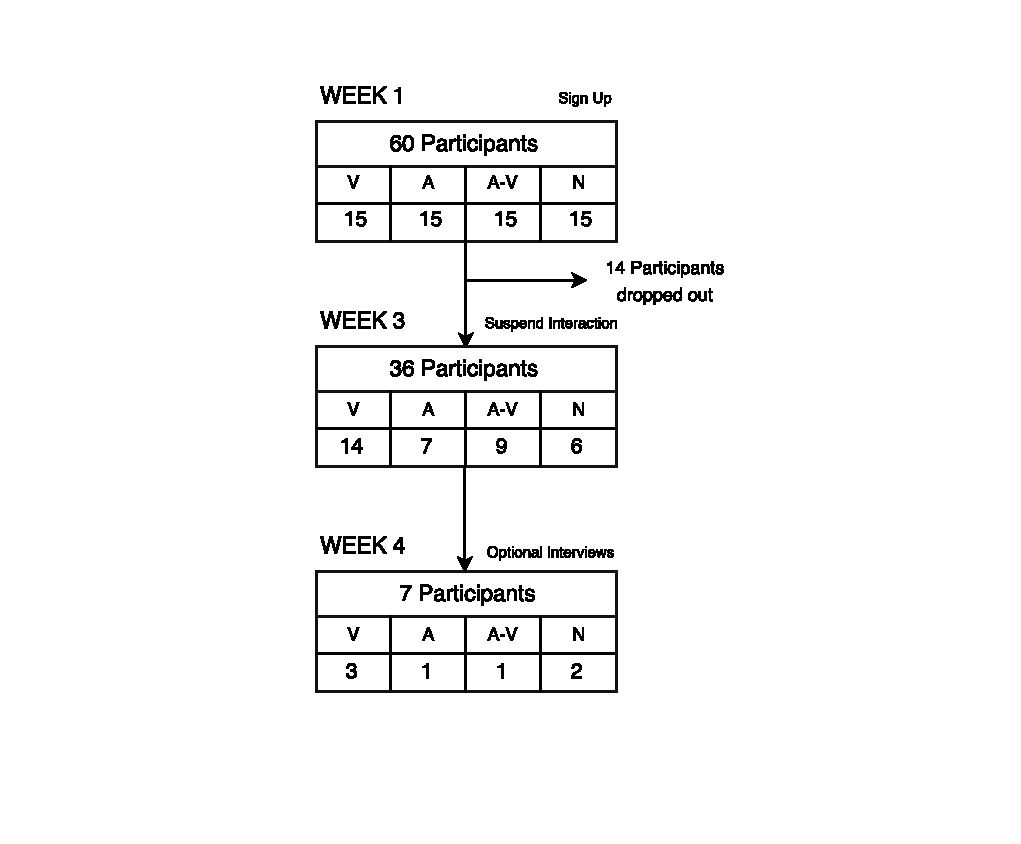
\includegraphics[width=.75\columnwidth]{figures/study-flow.pdf}
  \caption{Participant drop-out during the 4-week study. V: visual, A: auditory, V-A: visual-auditory, N: no rewards.}~\label{fig:study_dropout}
\end{figure}

\subsection{M1: Habit Performance}
Comparing the number of participants who dropped out of the study versus their reward modality, shows that 7 participants who blocked the bot had 27 visual rewards in total (mean = 3.85). 2 participants had 4 total auditory rewards (mean = 2) and 2 participants had 2 visual-auditory combined (mean = 6.5). These visual-auditory participants that dropped out had the highest amount of snoozes (24 total snoozes, 6 and 18 individually, mean = 12), compared with visual 10 total (mean = 2), and auditory with 0 snoozes.

7 participants (19\%) previously used habit tracking systems and 100\% of stated they worked well for tracking habits. These habits were: 'Diet' (3 mentions), 'Exercise' (3 mentions), 'Deadlines' (2 mentions), 'Audiobook reading' (1 mention), 'Weight' (1 mention). All of these participants chose new habits that they had not tracked before. Meditation was the most popular habit chosen (12 participants 33\%), followed by Press ups (8 participants 22\%), then Stretching (6 participants 15\%). Reading and writing were the least, only selected by 4 and 2 participants respectively. Stretching (6 participants 15\%) was the most completed habit based on selection (60 times), ranking 10.0 (where 10.0 = 60/6). Meditation ranked 6.25 (6.25 = 75/12) and the least were the plank and reading with 3.75 (15/4) and 1.75 (7/4) respectively.

Participants (14 participants 39\%) with visual rewards had the highest total number of snoozes (72 total presses to 'Not Yet'), auditory had the smallest (14 total). The control group had 55 snoozes and visual-auditory had 45 snoozes. Most participants snoozed (answered 'Not Yet') in the morning (100 times), specifically mid (66) and late (27) morning. Visual-auditory had the most number of failed snoozes (10, split over 6 participants, 1 person had 5 failed snoozes). Then it was auditory by 4.

Habit performance was also tracked in the form of a streak. If a participant did not track a habit for a day, their streak would be reset to 0. Meditation had the most cumulative streak (17) followed by stretching (7). High streaks (streak > 10) had habits: meditation (135 streaks) and stretch (126 streaks). Visual-auditory rewards had the most streaks (126), control group (75) and visual (60). Stretch had the highest peak streak (18), meditation (15). However, overall, for all completed habits, meditation was the most streaked (269), stretching (231), press ups (39) and plank (24).


\subsubsection{M1H1: The rewards effect on habit performance}

A one-way between-groups analysis of variance with planned comparisons was conducted to explore the effect of rewards on the number of habits completed, compared with the control group (Figure~\ref{fig:m1_h1}). Participants were divided into two groups according to their reward mode (Group 1: visual rewards, auditory rewards, visual-auditory rewards; Group 2: control group). There was a statistically significant difference at the p < .005 level in both groups for 2\/3 of the Weeks: Week 1, F (1, 23.20) = 9.48, p = .005, Week 2, F (1, 33.35) = 4.46, p = 0.42 and Week 3, F (1, 50) = 17.01, p < 0.005. The effect size for Week 1, Week 2 and Week 3 are large, calculated using eta squared, were 0.25, 0.39 and 0.43 respectively, this shows a large difference in the mean scores.

\subsubsection{M1H2: multiple modalities versus singular mode}
A one-way between-groups analysis of variance with planned comparisons was conducted to explore the effect of multiple modalities and singular modalities on the number of habits completed (Figure~\ref{fig:m1_h2}). Participants were divided into two groups according to their mode (Group 1: visual rewards, auditory rewards; Group 2: visual-auditory rewards). There was a statistically significant difference at the p < .005 level in Week 2 and Week 3, and lots in all groups: Week 1, F (1, 50) = 0.69, p = .410, Week 2, F (1, 50) = 23.04, p < .005 and Week 3, F (1, 50) = 8.85, p = .005. The effect size for Week 1, Week 2 and Week 3 are large, calculated using eta squared, were 0.25, 0.39 and 0.43 respectively, this shows a large difference in the mean scores.


\begin{figure}
  \centering
 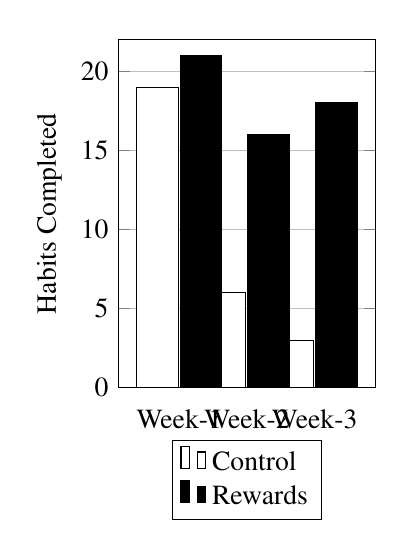
\begin{tikzpicture}
   \begin{axis}[
      width  = 0.4*\textwidth,
      height = 6cm,
      major x tick style = transparent,
      ybar=2*\pgflinewidth,
      bar width=15pt,
      ymajorgrids = true,
      symbolic x coords={Week-1, Week-2, Week-3},
      xtick = data,
      scaled y ticks = false,
      enlarge x limits=0.45,
      ymin=0,
      ymax=22,
      legend cell align=left,
      legend style={at={(0.5,-0.15)},anchor=north},
      ylabel={Habits Completed},
   ]
      \addplot[style={fill=white},error bars/.cd, y dir=both, y explicit]
          coordinates { % Control group
          (Week-1, 19)
          (Week-2, 6)
          (Week-3, 3)
          };

      \addplot[style={fill=black},error bars/.cd, y dir=both, y explicit,error bar style=red]
           coordinates { % Rewards
          (Week-1, 21)
          (Week-2, 16)
          (Week-3, 18)
           };

      \legend{Control, Rewards}

  \end{axis}
  \end{tikzpicture}
  \caption{M1H1: The rewards effect on habit performance. The sum of habits completed by participants with rewards versus the control group during 3-week study period.}~\label{fig:m1_h1}
\end{figure}


\subsection{M1: Habit Performance - Discussion}
The results found that participants are more likely to complete their habit if given one of the rewards whilst participants completed more habits with visual or auditory rewards than visual-auditory rewards.

\subsubsection{M1H1: The Rewards effect on Habit Performance}
There was a statistically significant drop in habit performance for the control group without rewards. This reveals the effect the rewards had on participant interaction with the bot and habit performance. The findings show that rewards did improve habit performance.

\subsubsection{M1H2: Multiple Modalities effect on Habit Performance}
There is a significant difference between the visual-auditory modes on the number of completed habits. But the result appears to be different to the initial hypotheses, with more participants completing habits with singular mode rewards than multiple. This contradicts the belief that multiple modalities benefits task completion, however these results only impact the particular rewards delivered by this bot. Therefore, it is inconclusive whether multiple modalities rewards in the general sense impact habit performance.

\subsection{M1: Habit Performance - Limitations and Future work}
This research relies on participants self-reporting and participants could have lied to remove the alert and get the reward. This is particularly true with the snooze function, as some participants found it annoying and stopped using the chatbot over time. They could have been simply getting rid of the reminder rather than completing the habit, therefore the measurement could have been how participants reacted to notifications, instead of their habit. Therefore, it is difficult to draw any valid conclusion on actual habit performance. Future work into how quickly participants responded to the alerts and if the device delivery (browser, iOS or Android) would better understand how participants interacted with the alerts.

\begin{figure}
  \centering
 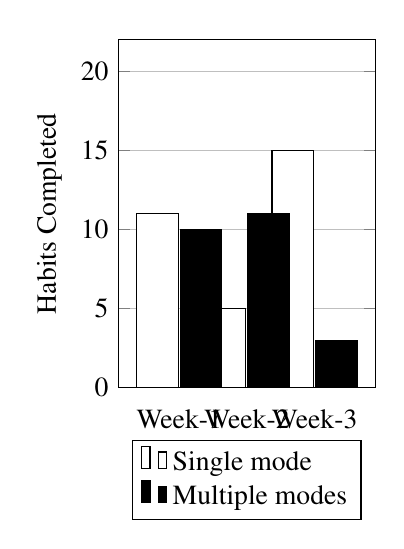
\begin{tikzpicture}
   \begin{axis}[
      width  = 0.4*\textwidth,
      height = 6cm,
      major x tick style = transparent,
      ybar=2*\pgflinewidth,
      bar width=15pt,
      ymajorgrids = true,
      symbolic x coords={Week-1, Week-2, Week-3},
      xtick = data,
      scaled y ticks = false,
      enlarge x limits=0.45,
      ymin=0,
      ymax=22,
      legend cell align=left,
      legend style={at={(0.5,-0.15)},anchor=north},
      ylabel={Habits Completed},
   ]
      \addplot[style={fill=white},error bars/.cd, y dir=both, y explicit,error bar style=red]
           coordinates { % Singular Modes
          (Week-1, 11)
          (Week-2, 5)
          (Week-3, 15)
           };

      \addplot[style={fill=black},error bars/.cd, y dir=both, y explicit]
          coordinates { % Multiple Modes
          (Week-1, 10)
          (Week-2, 11)
          (Week-3, 3)
          };

   
      \legend{Single mode, Multiple modes}

  \end{axis}
  \end{tikzpicture}
  \caption{M1H2: Multiple modes versus singular on habit performance. Sum of completed habits for multiple modalities compared with singular modes.}~\label{fig:m1_h2}
\end{figure}


\subsection{M2: Habit Automaticity}
11 participants completed both SRBAI questionnaires, 2 control group, 2 auditory, 5 visual and 2 visual-auditory. Out of these 11 participants, 7 participants volunteered for an interview. A paired-samples t-test was conducted to evaluate the change of habit automaticity between the first SRBAI questionnaire (after week 3) and the second (after week 4). There was a statistically significant increase in automaticity scores from SRBAI 1 (mean = 14.18, SD = 3.78) to SRBAI 2 (mean = 15.09, SD = 4.34), t (10) = 2.469, p < .005 (two-tailed). The mean increase in SRBAI scores was 0.90 with a 95\% confidence interval ranging from 0.08 to 1.72. The eta squared statistic (.37) indicated a large effect size.


\subsubsection{M2H1: the rewards effect on habit automaticity}
An independent-samples t-test was conducted to compare the habit automaticity scores
for rewards and control at both SRBAI 1 and SRBAI 2 (Figure~\ref{fig:m2_h1}). For SRBAI 1, there was also no significant differences in scores for rewards (mean = 14.33, SD = 3.84) and control (mean = 13.50, SD = 4.94; t (9) = 0.224, p = .85,
two-tailed). The magnitude of the differences in the means (mean difference = .83,
95\% CI: \-29.43 to 27.76) was very small (eta squared = .005). For SRBAI 2, there was no significant difference in scores for rewards
(mean = 15.22, SD = 4.29) and control (mean = 14.50, SD = 6.36; t (9) = 0.202, p = .84,
two-tailed). The magnitude of the differences in the means (mean difference = .72,
95\% CI: \-8.80 to 7.36) was very small (eta squared = .004).


A one-way between-groups analysis of variance with planned comparisons was also conducted to explore the impact of rewards on habit automaticity, as measured by the SRBAI 1 and 2. Participants were divided into two groups (Group 1: visual rewards, auditory rewards, visual-auditory rewards combined; Group 2: control group. There was not a
statistically significant difference for the two groups at SRBAI 1: F (1, 9) = 0.02, p = .88, and SRBAI 2: F (1, 9) = 0.07, p = .78. In addition, the difference in mean scores between the groups had, at SRBAI 1: a medium effect with an effect size of .11, and at SRBAI 2: a large effect, with an effect size of .17, both calculated using eta squared.



\subsubsection{M2H2: multiple modes versus singular mode on habit automaticity}
A one-way between-groups analysis of variance with planned comparisons was conducted to explore the
impact of multiple modalities on habit automaticity, compared with singular modes as measured by the SRBAI 1 and 2 (Figure~\ref{fig:m2_h2}). Participants were divided into two groups according to their reward mode (Group 1: visual rewards, auditory rewards; Group 2: visual-auditory combined rewards). There was not a
statistically significant difference for the two groups at SRBAI 1: F (1, 9) = 1.04, p = .33, and SRBAI 2: F (1, 9) = 0.64, p = .44. In addition, the difference in mean scores between the groups had, at SRBAI 1: a medium effect with an effect size of .11, and at SRBAI 2: a large effect, with an effect size of .17, both calculated using eta squared.




%       S1 Mean S2 Mean S1 SD   S2 SD
% Control 13.5  14.5  4.949747468 6.363961031
% Rewards 14.33 15.22 3.840572874 4.294699576

\begin{figure}
  \centering
 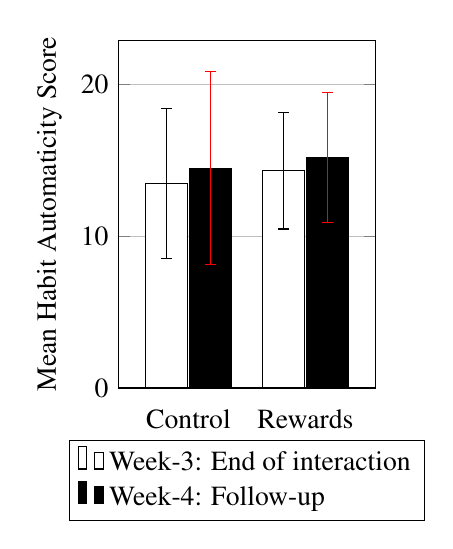
\begin{tikzpicture}
   \begin{axis}[
      width  = 0.4*\textwidth,
      height = 6cm,
      major x tick style = transparent,
      ybar=2*\pgflinewidth,
      bar width=15pt,
      ymajorgrids = true,
      symbolic x coords={Control,Rewards},
      xtick = data,
      scaled y ticks = false,
      enlarge x limits=0.60,
      ymin=0,
      legend cell align=left,
      legend style={at={(0.5,-0.15)},anchor=north},
%       x label style={at={(axis description cs:0.5,-0.1)},anchor=north},
%       y label style={at={(axis description cs:-0.1,.5)},rotate=90,anchor=south},
%       xlabel={$u$ unemployment},
      ylabel={Mean Habit Automaticity Score},
   ]
      \addplot[style={fill=white},error bars/.cd, y dir=both, y explicit]
          coordinates {
          (Control, 13.5) += (0,4.94) -= (0,4.94)
          (Rewards, 14.33) += (0,3.84) -= (0,3.84)
          };

      \addplot[style={fill=black},error bars/.cd, y dir=both, y explicit,error bar style=red]
           coordinates {
           (Control, 14.5) += (0,6.36) -= (0,6.36)
           (Rewards, 15.22) += (0,4.29) -= (0,4.29)
           };

      \legend{Week-3: End of interaction, Week-4: Follow-up}

  \end{axis}
  \end{tikzpicture}
  \caption{M2H1: The rewards effect on habit automaticity. Comparing mean habit automaticity for rewards versus control group.}~\label{fig:m2_h1}
\end{figure}



\subsection{Interview Feedback}
The interview transcripts were analysed and participants were anonymised following a thematic approach~\cite{thematic_analysis_qualatitive_data}. Below, we consider the role of each participants during the process of interacting with the chatbot and reflect how their interaction may of had a meaningful impact to their formation of a new habit.

7 interviews with participants outlined their experience with their habit performance after the prototype bot was removed. Participants picked habits they wanted to perform, but when the bot stopped notifying them, they lacked motivation to completed their habit. Some participants enjoyed the rewards at the beginning, but most participants disliked them after the first week.

Participants discussed how they picked their habit, they chose because they had wanted to start for the particular habit for a long time, it was \textit{'not too much effort'} and \textit{'something successful people do'}. They wanted \textit{'to be more active'}, \textit{'relieve stress'} and wanted a habit that was \textit{'less time consuming'}. Throughout, participants mostly completed their habits, but, some participants would put the message off and eventually their performance would get \textit{'worse and worse'} until they stopped all together. However, after the bot was removed all interviewed participants (N = 7) found it difficult to continue with their habit. They \textit{'kept forgetting'}, found it \textit{'harder to remember'} and lacked motivation, not performing the action if it had \textit{'been a long day'}. Some tried to do it \textit{'every now and again'}, but usually they would only complete it if \textit{'they remembered'}. This reveals the dependency between technology and habits, suggesting that the bot did not increase habit automaticity, or that the existing routine participants chose was not suitable for new habits, or that they were not given enough time to develop automaticity.


%       S1 Mean S2 Mean S1 SD S2 SD
% Visual  14.6  15.8  4.336 3.701
% Auditory  12    11.5  4.243 6.364
% V-A   16    17.5  2.828 3.536

\begin{figure}
  \centering
 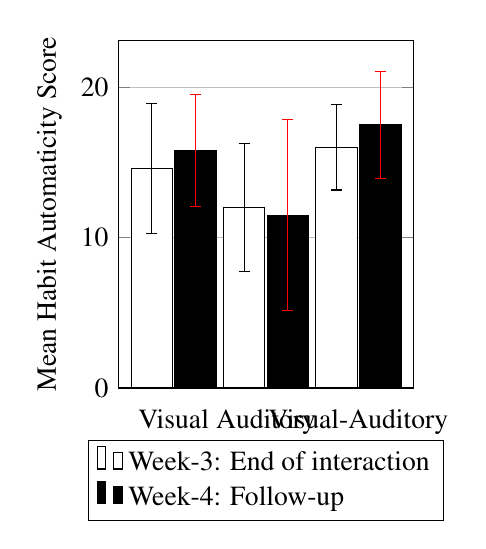
\begin{tikzpicture}
   \begin{axis}[
      width  = 0.44*\textwidth,
      height = 6cm,
      major x tick style = transparent,
      ybar=2*\pgflinewidth,
      bar width=15pt,
      ymajorgrids = true,
      symbolic x coords={Visual,Auditory,Visual-Auditory},
      xtick = data,
      scaled y ticks = false,
      enlarge x limits=0.3, % how far apart the bars are
      ymin=0,
      legend cell align=left,
      legend style={at={(0.5,-0.15)},anchor=north},
%       x label style={at={(axis description cs:0.5,-0.1)},anchor=north},
%       y label style={at={(axis description cs:-0.1,.5)},rotate=90,anchor=south},
%       xlabel={$u$ unemployment},
      ylabel={Mean Habit Automaticity Score},
   ]
      \addplot[style={fill=white},error bars/.cd, y dir=both, y explicit]
          coordinates {
          (Visual, 14.6) += (0,4.336) -= (0,4.336)
          (Auditory, 12) += (0,4.243) -= (0,4.243)
          (Visual-Auditory, 16) += (0,2.828) -= (0,2.828)
          };

      \addplot[style={fill=black},error bars/.cd, y dir=both, y explicit,error bar style=red]
           coordinates {
          (Visual,15.8) += (0,3.701) -= (0,3.701)
          (Auditory, 11.5) += (0,6.364) -= (0,6.364)
          (Visual-Auditory, 17.5) += (0,3.536) -= (0,3.536)
           };

      \legend{Week-3: End of interaction, Week-4: Follow-up}

  \end{axis}
  \end{tikzpicture}
  \caption{M2H2: Multiple modes versus singular on habit performance. Comparing mean habit automaticity for each group.}~\label{fig:m2_h2}
\end{figure}

Participants had mixed feelings about the rewards. Some \textit{'did not like the [visual] rewards'}, skipping over them after the first few, they \textit{'just wanted to get rid of the notification dot'}. Another participant said \textit{'some of them [visual-auditory rewards] were funny'}, but they did not like them overall and mentioned the auditory rewards were \textit{'too random'}. One participant thought they did not give them an incentive towards their habit, just a \textit{'nice little extra'}. They also discussed including time-sensitive rewards, as they did not want to listen to music before going to bed. This shows the importance of using an appropriate modality at particular times, e.g. not having auditory rewards at certain times of the day. Finally, an upbeat participant talked about \textit{'always wanting to open them'} and \textit{'the combination was perfect'}. However, they said they also found them \textit{'repetitive'}.


Participants were asked about how they found the chatbot as the method of interaction. They found the method \textit{'pretty good'}, they \textit{'liked it'} and \textit{'would have liked more interaction'}. Suggesting additional features, such as \textit{'help and support throughout'}, \textit{'ideas on how to improve your habit'} and \textit{'advice on how to set aside time for your habit'}. Others were neutral, some expecting \textit{'different messages, such as Hey [name], a bit more care about the person, a bit less like a robot'}. Lots of participants (N = 4) enjoyed the reminder aspect, but a few found it \textit{'repetitive'} and \textit{'got annoying if I pressed Not Yet'}. Participants wanted to see their progress as they tracked their habits, they talked about wanting to reflect on their data. They mentioned that they would feel \textit{'more encouraged to keep doing it, rather than random music [auditory rewards]'}.


Mostly participants wanted the prototype to come back with a few modifications: \textit{'enclosed with Fitbit so it is all in a single place'}, \textit{'fine without rewards'} (2 participants mentioned this), \textit{'more interaction'} and \textit{'with statistics about my progress'}. Participants wanted the bot as more of a \textit{'constant persistent reminder'} with additional tracking elements to remind them to perform their habit to fit into their busy schedule. Participants (N = 5) mentioned the \textit{headspace} app (\url{www.headspace.com}), mentioning that they wanted a combination of the bot and headspace. It prompted another participant to download the headspace app. They wanted the bot to keep on track of their habit and they would use the headspace app to help them perform their mindfulness.


\subsection{M2: Habit Automaticity - Discussion}
It is inconclusive whether the rewards or the combined modalities effected habit automaticity. 

\subsubsection{M2H1: The Rewards effect on Habit Automaticity}
Each individual reward did not have a significant effect on habit automaticity. Although participants with rewards had slightly higher automaticity scores and follow up interviews suggest that automaticity did not develop with participants discussing negative feelings towards rewards during the interviews.  

\subsubsection{M2H2: Multiple Modalities effect on Habit Automaticity}
Participants with visual-auditory combined reward had higher habit automaticity scores compared with visual or auditory rewards. However, these were not statistically significant.

\subsection{M2: Habit Automaticity - Limitations and Future work}
Only 7 participants responded to the follow up interviews. In addition, the study relied on participants recall which could be inaccurate. Future work conducting similar research with a larger sample size for the SRBAI questionnaire would validate these findings

\section{General Discussion}
This research aimed to understand more about rewards from different modalities and their role in habit formation. Participants receiving bot-delivered rewards completed more habits than the control group without rewards. There was a significant correlation between the habit formation method and habit automaticity. However, this was contradicted during participant interviews (N = 7) where all participants found a drop in habit performance after 1-week without the prototype.

% Under half the participants completed the modality survey (N = 12, 40\%). These had the following rewards: visual rewards had the highest score (the higher, the more participants preferred the reward) (mean = 12, SD = 3.347), visual and auditory rewards were slightly below (mean = 10.75, SD = 1.893).
% TODO: Compare these results to people not using the chatbot, e.g.. people signing up to the gym, new years resolution

\subsection{Prototype Success}
The prototype was somewhat successful at running a research trial. There were several issues and various limitations with development. However, it was generally liked by participants and managed to easily gather a lot of useful data.

Participants had mixed feelings towards the bot. Their performance shows that the number of snoozes over time decreased, but the number of total habits completed per day also decreased for all reward types (including the control group). However, participant streaks over time increased and 36 participants manage to use it for 3-weeks.

Participants had various issues with bot interaction. 7 participants tried to message the bot during setup, instead of using the built in \textit{quick reply} buttons. This broke the setup flow and they had to start again. Other participants tried to send multiple messages when asked for free input, they went around an endless loop when asking for a habit type and participants tried to mark their habit as completed using the Facebook Messenger thumb emotion (which the bot was not coded for).

Participants gave additional feedback by simply messaging the bot. They asked inquisitive questions, such as \textit{'what kind of thing are you looking to find out'}, \textit{'this is not working for me'} and \textit{'stop'}---to try and stop the daily messages (the participant then blocked the bot). Negative feedback towards the rewards and bot were also expressed. When asked about being messaged every day, a participant sent this reply and then blocked the bot: \textit{'Do not do that, it will be annoying'}, and another said \textit{'never message me'}. Another stated that this was the \textit{'lame same band'} after receiving a auditory reward.

Mostly participants chose existing routines that were suggested to them. For example, during the pilot trials when asking for an existing routine, users were confused, so examples of habit contexts were provided. The results found, 31 (84\%) participants chose one of the contexts that were listed as examples, some with a slight change in before and after wording, e.g. \textit{before} getting home from work, rather than \textit{after} getting home from work. The remaining 5 participants chose the following context: \textit{'Having a snack'}, \textit{'Sitting in bed'}, \textit{'Early morning'}, \textit{'During breakfast'} and \textit{'Before sleeping'}. A participant also pointed out that they could change their existing routine time but were unable to change the description.

\subsection{Dependence}
Streaks could have been better used to give insight to participants progress and challenged them to maintain it, using loss aversion~\cite{loss_aversion} to compare the impact of their broken streak with the gain of keeping it. However, all participants interviewed (N = 7) struggled with maintaining habit performance after the bot was removed. This suggests a dependence between the technology and the habit as participants depended on bot notifications to continue repeating the desired action.

\subsection{General Limitations and Future Work}
This research has four key limitations. First, the small number of participants and the small sample of rewards used in the study make it unclear how these findings would generalise to other types of rewards with the same modality. Second, this only applies to intrinsic positive reinforcement rewards, further research into how different types of rewards from different modalities is needed. Third, dependency between the prototype and participants habit performance during the 3-week period is outlined and how this has disadvantages for habit formation. Finally, the content and method of delivery is another variable that effects these results, additional studies into bot-delivered rewards would validate these findings. 

\section{Conclusions}
The results found that the bot-delivered rewards improved habit performance. Participants were more likely to complete their habit if given the reward. Habit performance was also effected by different modalities, although not in the way our hypotheses assumed, as singular modalities had higher habit performance than visual-auditory rewards. Finally, the limitations of the study do not show any clear statistical significance whether the rewards or the combined modalities effected habit automaticity. More conclusive evidence is needed to show that rewards from combined modalities effect habit automaticity. Using these results to compare different types of visual, auditory and visual-auditory rewards with behaviour change technology may open up new research avenues for investigating the use of bots as tools to help form new habits.

\section{Acknowledgements}
Thank you to all the participants involved, the internal reviewers and staff who provided helpful feedback throughout the study.

\balance{}

% % Either:
% %  1. Put \balance in the first column of the last page
% %  2. Don't use \balance
% %  3. hard-code a column break into the bbl file (before submission)
% % see more http://stackoverflow.com/questions/2149854/how-to-manually-equalize-columns-in-an-ieee-paper-if-using-bibtex
% \balance{}


\bibliographystyle{scaffold/SIGCHI-Reference-Format}
\bibliography{sample}

\end{document}
